\subsection{Walidacja krzyżowa}
\subsubsection{Metoda zbioru walidacyjnego}
Na początku wczytuję dane, usuwam wartości NaN i przygotowuję zbiór walidacyjny.

\begin{Rcode}
energy_data <- read.csv("energy_dataset.csv")
energy_data <- na.omit(energy_data)
set.seed(1)
n <- nrow(energy_data)
train <- sample(n, n / 2)
\end{Rcode}
Dopasowuję model liniowy na zbiorze uczącym i obliczam MSE dla zbioru walidacyjnego:

\begin{Rcode}
energy_lm <- lm(Type_of_Renewable_Energy ~ Energy_Production_MWh,
                 data = energy_data,
                 subset = train)

validation_set <- energy_data[-train,]

mse <- mean((validation_set$Type_of_Renewable_Energy -
              predict(energy_lm, validation_set))^2)

\end{Rcode}
Otrzymana wartość MSE: \textbf{4.0439057662439}.

Użyjmy wielomianów o różnych stopniach:

\end{Rcode}
Dopasowuję model liniowy na zbiorze uczącym i obliczam MSE dla zbioru walidacyjnego:

\begin{Rcode}
for (i in 2:5) {
  energy_lm_poly <- lm(Type_of_Renewable_Energy ~ poly(Energy_Production_MWh, degree = i), data = energy_data, 
                     subset = train)
  print(mean((validation_set$Type_of_Renewable_Energy - predict(energy_lm_poly, validation_set))^2))
}
\end{Rcode}
Otrzymujemy MSE: 

\begin{Rcode}
[1] 4.042959
[1] 4.041494
[1] 4.041374
[1] 4.042979
\end{Rcode}
\textbf{Wniosek} - stopień wielomianu w tym przypadku nie ma znaczącego wpływu na otrzymany MSE.
Powtarzam obliczenia dla innego zbioru walidacyjnego:

\begin{Rcode}
degree_max <- 5

compute_mse <- function(degree, train) {
  energy_lm <- lm(Type_of_Renewable_Energy ~ poly(Energy_Production_MWh, degree), data = energy_data, subset = train)
  validation_set <- energy_data[-train,]
  mean((validation_set$Type_of_Renewable_Energy - predict(energy_lm, validation_set))^2)
}

mse <- vapply(1:degree_max, compute_mse, FUN.VALUE = numeric(1), train = train)
\end{Rcode}
Otrzymane wartości MSE:
\begin{Rcode}
4.04390576624393
4.04295881295649
4.04149420436449
4.04137383913034
4.04297885010734
\end{Rcode}

\begin{figure}[H]
    \centering
    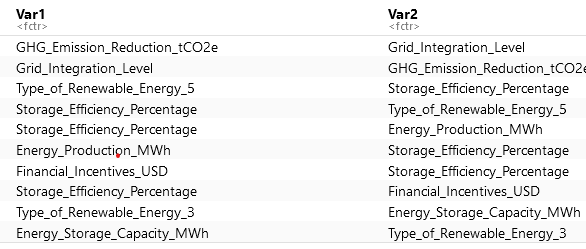
\includegraphics[width=0.8\linewidth]{lab3/obraz.png}
    \caption{Zależność między wartością MSE a stopniem wielomianu.}
    \label{fig:enter-label}
\end{figure}

\subsubsection{Walidacja krzyżowa bez jednego (leave-one-out)}

\begin{Rcode}
set.seed(2)
train <- sample(n, n / 2)
validation_set <- energy_data[-train,]
degree_max <- 10
mse <- rep(0, times = degree_max)
for (i in 1:degree_max) {
  energy_lm <- lm(Type_of_Renewable_Energy ~ poly(Energy_Production_MWh, degree = i), data = energy_data, subset = train)
  mse[i] <- mean((validation_set$Type_of_Renewable_Energy - predict(energy_lm, validation_set))^2)
}
mse
\end{Rcode}

\begin{Rcode}
    TUTAJ WYKRES TEGO WYZEJ
\end{Rcode}

\begin{Rcode}
[Co teraz z wnioskami na temat regresji wielomianowej w naszym przypadku?]
[Sprawdź, że dla LOOCV obie współrzędne delta zawierają praktycznie to samo.]
\end{Rcode}

\subsubsection{K-krotna walidacja krzyżowa}
Tym razem jawnie ustawiamy parametr K oznaczający liczbę grup:

\begin{Rcode}
compute_kcv_mse <- function(degree, k) {
    energy_glm <- glm(Type_of_Renewable_Energy ~ poly(Energy_Production_MWh, degree), data = energy_data)
    cv.glm(energy_data, energy_glm, K = k)$delta[1]
}
mse <- sapply(1:degree_max, compute_kcv_mse, k = 10)
\end{Rcode}
Zestawiamy 10 wyników:
\begin{Rcode}
mse10 <- replicate(10, sapply(1:degree_max, compute_kcv_mse, k = 10))
\end{Rcode}
Otrzymujemy:
\begin{Rcode}
    10 WYNIKOW
\end{Rcode}
\begin{Rcode}
    WYKRES
\end{Rcode}
\begin{Rcode}
    CO Z WYNIKAMI
\end{Rcode}

\subsubsection{Bootstrap}
Użyjmy metody bootstrap do oszacowania błędów standardowych współczynników regresji liniowej.

\begin{Rcode}
lm_coefs <- function(data, index = 1:nrow(data)) {
  coef(lm(Type_of_Renewable_Energy ~ Energy_Production_MWh, data = energy_data, subset = index))
}

n <- nrow(energy_data)
lm_coefs(energy_data, sample(n, n, replace = TRUE))

lm_coefs(energy_data)

boot(energy_data, lm_coefs, R = 1000)
}
\end{Rcode}

W ten sposób obliczyliśmy błąd standardowy z 1000 replikacji.

\begin{figure}[H]
    \centering
    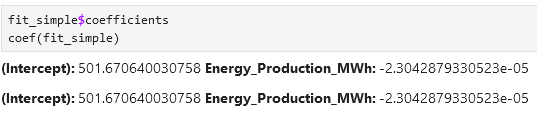
\includegraphics[width=1\linewidth]{lab3/obraz2.png}
    \caption{Wyniki dla regresji liniowej z użyciem metody boostrap}
    \label{fig:enter-label}
\end{figure}

Powtórzmy eksperyment dla regresji kwadratowej:

\begin{Rcode}
lm_coefs <- function(data, index = 1:nrow(data)) {
  coef(lm(Type_of_Renewable_Energy ~ (Energy_Production_MWh)^2, data = energy_data, subset = index))
}

n <- nrow(energy_data)
lm_coefs(energy_data, sample(n, n, replace = TRUE))

lm_coefs(energy_data)

boot(energy_data, lm_coefs, R = 1000)
\end{Rcode}

\begin{figure}[H]
    \centering
    \includegraphics[width=1\linewidth]{lab3/obraz2_5.png}
    \caption{Wyniki dla regresji kwadratowej z użyciem metody boostrap}
    \label{fig:enter-label}
\end{figure}

\subsection{Selekcja cech dla modeli liniowych}
Podzielmy nasz główny zbiór na podzbiory za pomocą metody \textit{regsubsets}. Wykorzystamy wszystkie 12 zmiennych objaśniających

\begin{Rcode}
energy_bs <- regsubsets(Type_of_Renewable_Energy ~ ., data = energy_data, nvmax=12)
energy_bs_sum <- summary(energy_bs)
energy_bs_sum
\end{Rcode}

Sprawdźmy, który predyktor zagwarantuje mam najlepszy podzbiór. Używamy metryki \textbf{BIC}, która powinna być jak najmniejsza.

\begin{Rcode}
energy_bs_sum$cp
bic_min <- which.min(energy_bs_sum$bic)
bic_min
energy_bs_sum$bic[bic_min]

energy_bs_sum

plot(energy_bs_sum$bic, xlab = "Liczba zmiennych", ylab = "BIC", col = "green",
     type = "b", pch = 20)
points(bic_min, energy_bs_sum$bic[bic_min], col = "red", pch = 9)

plot(energy_bs, scale = "bic")    
\end{Rcode}

\begin{figure}[H]
    \centering
    \includegraphics[width=1\linewidth]{lab3/obraz3_5.png}
    \caption{Liczba zmiennych a wartość BIC}
    \label{fig:enter-label}
\end{figure}

\begin{figure}[H]
    \centering
    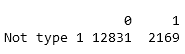
\includegraphics[width=1\linewidth]{lab3/obraz3.png}
    \caption{Ocena predyktorów}
    \label{fig:enter-label}
\end{figure}

Najlepszym wyborem zdaje się być \textbf{grid\_integration\_level}.

Estymaty parametrów dla optymalnego podzbioru:

\begin{Rcode}
coef(energy_bs, id = 8)
\end{Rcode}

\begin{figure}[H]
    \centering
    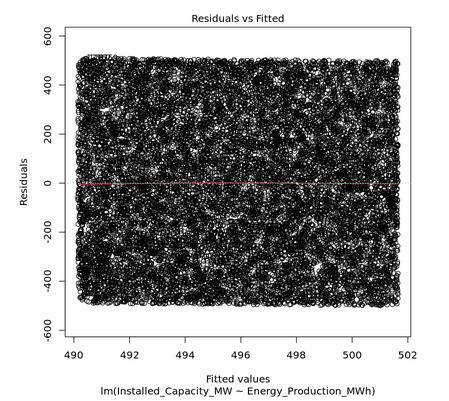
\includegraphics[width=1\linewidth]{lab3/obraz4.png}
    \caption{Podusmowanie dla metryki BIC}
    \label{fig:enter-label}
\end{figure}

Wykorzystajmy jeszcze metrykę \textbf{$R^2$}, zaimplementowaną analogicznie do BIC.

\begin{figure}[H]
    \centering
    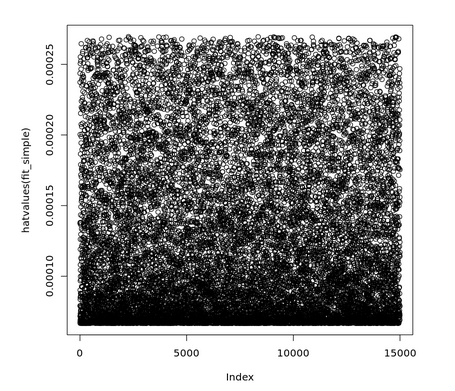
\includegraphics[width=1\linewidth]{lab3/obraz6.png}
    \caption{Liczba zmiennych a wartość $R^2$}
    \label{fig:enter-label}
\end{figure}

\begin{figure}[H]
    \centering
    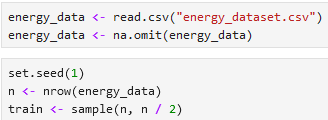
\includegraphics[width=1\linewidth]{lab3/obraz7.png}
    \caption{Ocena predyktorów}
    \label{fig:enter-label}
\end{figure}

Według metryki $R^2$, najlepszymi predyktorami są \textbf{Initial\_Investment\_USD} i \textbf{GHG\_Emission\_Reduction\_tCO2e}.

\subsubsection{Selekcja krokowa do przodu i wstecz}
Używamy teraz selekcji krokowej

\begin{Rcode}
energy_fwd <- regsubsets(Type_of_Renewable_Energy ~ ., data = energy_data, nvmax=10, 
                          method = "forward")
energy_fwd_sum <- summary(energy_fwd)
energy_fwd_sum
energy_back <- regsubsets(Type_of_Renewable_Energy ~ ., data = energy_data, nvmax=10, 
                          method = "backward")
energy_back_sum <- summary(energy_back)
energy_back_sum
\end{Rcode}

\begin{figure}[H]
    \centering
    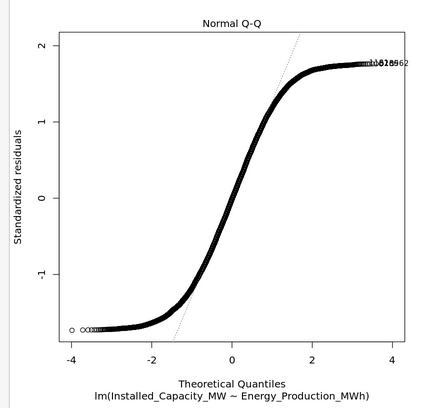
\includegraphics[width=1\linewidth]{lab3/obraz5.png}
    \caption{Enter Caption}
    \label{fig:enter-label}
\end{figure}

\subsubsection{Wybór modelu przy pomocy metody zbioru walidacyjnego}

\begin{Rcode}
n <- nrow(energy_data)
train <- sample(c(TRUE, FALSE), n, replace = TRUE)
test <- !train
energy_bs_v <- regsubsets(Type_of_Renewable_Energy ~ ., data = energy_data, nvmax=10)
\end{Rcode}

\begin{Rcode}
predict.regsubsets <- function(object, newdata, id, ...) {
  model_formula <- as.formula(object$call[[2]])
  mat <- model.matrix(model_formula, newdata)
  coefs <- coef(object, id = id)
  mat[, names(coefs)] %*% coefs
}
\end{Rcode}

\begin{Rcode}
prediction_error <- function(i, model, subset) {
pred <- predict(model, energy_data[subset,], id = i)
mean((energy_data$Type_of_Renewable_Energy[subset] - pred)^2)
}
val_errors <- sapply(1:10, prediction_error, model = energy_bs_v, subset = test)
val_errors   
\end{Rcode}

Otrzymaliśmy takie wartości błędu: 
\begin{Rcode}
4.013148 4.012435 4.012165 4.011892 4.011292 4.011261 4.011174 4.010870 4.010838 4.010614
\end{Rcode}
Możemy więc wywnioskować, że optymalny model ma 10 parametrów.

\subsubsection{Wybór modelu przy pomocy k-krotnej walidacji krzyżowej}

\begin{Rcode}
k <- 10
folds <- sample(1:k, n, replace = TRUE)
val_err <- NULL
for (j in 1:k) {
  fit_bs <- regsubsets(Type_of_Renewable_Energy ~ ., data = energy_data[folds != j,], nvmax=10)
  err <- sapply(1:10, prediction_error, model = fit_bs, subset = (folds == j))
  val_err <- rbind(val_err, err)
}

cv_errors <- colMeans(val_err)
cv_errors
\end{Rcode}

Otrzymaliśmy takie wartości błędów:

\begin{Rcode}
3.998710 3.996294 3.998936 3.999858 4.000146 4.000639 4.000911 4.000728 4.000925 4.000906
\end{Rcode}

Według tego kryterium, optymalny model powinien mieć dwa parametry.